%ju 28-Mai-22 FM_U04_Spannungsabfall_Loesung.tex
\section{Spannungsabfall Übung 4}\label{spannungsabfall-uebung-4}

Tabellenbuch S. 280 Nennquerschnitt

\textbf{Aufgabe 1}

geg:

$A = 0,6~mm^2$

$\rho = 0,3~\frac{\Omega \cdot mm^2}{m}$

$I = 8~A$

$U_v = 4~V$

ges: $l$

Formel:

$U_v = \frac{\rho \cdot l \cdot I}{A} \to l = \frac{U_v \cdot A}{\rho \cdot I}$

Lösung:

$l = 1,0~m$

\textbf{Aufgabe 2}

geg:

$l = 4~m$ (Kupfer)

$U_{ges} = 10~V, U_k = 9,6~V$

$I = 150~A$

$\rho = 0,0178~\frac{\Omega \cdot mm^2}{m}$

ges: $R_{st}, A_{mind}, A_{Nenn}$

Formel:

$R_{st} = \frac{U_k}{I}$

$U_v = U_{ges} - U_k \to A_{mind} = \frac{\rho \cdot l \cdot I}{U_v} \to A_{mind} = \frac{\rho \cdot l \cdot I}{(U_{ges} - U_k)}$

Lösung:

$R_{st} = 0,064~\Omega$

$A_{mind} = 26,7~mm^2 \to A_{Nenn} = 35~mm^2$ (Nennquerschnitt)

\newpage

\textbf{Aufgabe 3}

geg:

$A = 0,75~mm^2$

$l = 6~m$ (Kupfer)

$U_v = 0,3~V = 300 mV$

$\rho = 0,0178~\frac{\Omega \cdot mm^2}{m}$

ges: $I$

Formel:

$U_v = \frac{\rho \cdot l \cdot I}{A} \to I = \frac{U_v \cdot A}{\rho \cdot l}$

Lösung:

$I = 2,1067~A$

\textbf{Aufgabe 4}

\begin{figure}[!ht]% hier: !ht
\centering
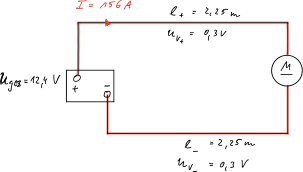
\includegraphics[width=0.6\textwidth]{images/Skizze/24_FM_Nr4_Reihenschaltung_Aufg4_Skizze.pdf}
\caption{Schaltung Spannungsabfall Aufgabe 4}
%\label{fig:}%% anpassen
\end{figure}

geg:

$l = 4,5~m$ (Kupfer), $l_1 = 2,25~m$ (Plusleitung), $l_2 = 2,25~m$
(Minusleitung)

$U_v = 0,3~V, U_B = 12,4~V$

$\rho = 0,0178~\frac{\Omega \cdot mm^2}{m}$

$I = 156~A$

ges: $R_{st}, A_{mind}, A_{Nenn}$

Formel:

$U_k = U_B - U_{v_+} - U_{v_-} \to R_{st} = \frac{U_k}{I} \to R_{st} = \frac{(U_B - U_{v_+} - U_{v_-})}{I}$

$U_v = \frac{\rho \cdot l \cdot I}{A} \to A_{mind} = \frac{\rho \cdot l_1 \cdot I}{U_v}$

Lösung:

$R_{st} = 0,0756~\Omega$

$A_{mind} = 20,826~mm^2 \to A_{Nenn} = 25~mm^2$ (Nennquerschnitt)

\newpage

\textbf{Aufgabe 5}

geg:

$l = 1,65~m$ (Kupfer)

$U_{v_\%} = 2,5~\% \text{ von } 12~V$

$U_{ges} = 12~V$

$\rho = 0,0178~\frac{\Omega \cdot mm^2}{m}$

$I = 50~A$

ges: $U_v, A_{mind}, A_{Nenn}$

Formel:

$U_{v_\%} = \frac{U_v \cdot 100}{U_{ges}} \to U_v = \frac{U_{v_\%} \cdot U_{ges}}{100}$

$U_v = \frac{\rho \cdot l \cdot I}{A} \to A_{mind} = \frac{\rho \cdot l \cdot I}{U_v}$

Lösung:

$U_v = 0,3~V$

$A_{mind} = 4,895~mm^2 \to A_{Nenn} = 6~mm^2$ (Nennquerschnitt)

\textbf{Aufgabe 6}

geg:

$U_v = 0,10385232~V = 103,85232~mV$

$\rho = 0,0178~\frac{\Omega \cdot mm^2}{m}$

$I = 1,87~A$

$A = 1,5~mm^2$

ges: $l$

Formel:

$U_v = \frac{\rho \cdot l \cdot I}{A} \to l = \frac{U_v \cdot A}{\rho \cdot I}$

Lösung:

$l = 4,68~m$
